\documentclass[11pt,a4paper]{report}

\usepackage[utf8]{inputenc}
\usepackage{amsmath}
\usepackage{graphicx}
\usepackage{gensymb}
\usepackage{tikz}
\usepackage{pgfplots}
\usetikzlibrary{positioning}
\usepackage{geometry}
\geometry{
    left=2cm,
    right=0.64cm,
    top=0.64cm,
    bottom=2cm
}
\usepackage{multicol}
\setlength{\columnsep}{1cm}
\graphicspath{ {images/} }

\begin{document}

\chapter{Semester 2 Examination 2015-2016\\CZ4041 Machine Learning}

\begin{multicols*}{2}

\section{Question 1}
\noindent \textbf{Question 1a}
\noindent Information given in the question:
\begin{itemize}
  \item $P(D) = 0.001$
  \item $P(\sim D) = 0.999$
  \item $P(T_1|D) = 0.9$
  \item $P(T_2|D) = 0.95$
  \item $P(T_1|\sim D) = 0.01$
  \item $P(T_2|\sim D) = 0.1$
\end{itemize}

\begin{equation*}
\begin{split}
P(D|T_1 T_2) &= \frac{P(T_1 | D) P(T_2 | D) P(D)}{P(T_1 T_2)}\\
&= \frac{0.9 \times 0.95 \times 0.001}{P(T_1 T_2)}\\
&= \frac{0.855 \times 10^{-3}}{P(T_1 T_2)}
\end{split}
\end{equation*}

\begin{equation*}
\begin{split}
P(\sim D|T_1 T_2) &= \frac{P(T_1 | \sim D) P(T_2 | \sim D) P(\sim D)}{P(T_1 T_2)}\\
&= \frac{0.01 \times 0.1 \times 0.999}{P(T_1 T_2)}\\
&= \frac{0.999 \times 10^{-3}}{P(T_1 T_2)}
\end{split}
\end{equation*}

\noindent Since $P(\sim D|T_1 T_2) > P(D|T_1 T_2)$, we predict that the patient does not have the disease.\\

\noindent \textbf{Question 1b}

\noindent Let action $a_1$ be the action predicting the patient to have the disease, and action $a_2$ be the action predicting the patient to not have the disease.

$$R(a_1|T_1 T_2) = 1 - P( D | T_1 T_2)$$
$$R(a_2|T_1 T_2) = 1 - P( \sim D | T_1 T_2)$$

\noindent We choose the action with minimum risk. Since $P(\sim D|T_1 T_2) > P(D|T_1 T_2)$, thus $R(a_2|T_1 T_2) < R(a_1|T_1 T_2)$, so the action $a_2$ has lower risk. As a result, we predict that the patient does not have the disease.\\

\noindent \textbf{Question 1c}

\noindent Information given in the question:
\begin{itemize}
  \item $\lambda_{12} = 0.05$
  \item $\lambda_{21} = 1$
\end{itemize}

\noindent Where $\lambda_{12}$ is the lost occur when the action is predict the patient to have disease $a_1$, but the ground truth is the patient do not have the disease $\sim D$. The lost $\lambda_{21}$ is defined in similar way. The risks are:

\begin{equation*}
\begin{split}
R(a_1|T_1 T_2) &= \lambda_{12} P(\sim D | T_1 T_2)\\
&= 0.05 \times \frac{0.999 \times 10^{-3}}{P(T_1 T_2)}\\
&= \frac{0.4995 \times 10^{-3}}{P(T_1 T_2)}
\end{split}
\end{equation*}

\begin{equation*}
\begin{split}
R(a_2|T_1 T_2) &= \lambda_{21} P( D | T_1 T_2)\\
&= 1 \times \frac{0.855 \times 10^{-3}}{P(T_1 T_2)}\\
&= \frac{0.855 \times 10^{-3}}{P(T_1 T_2)}\\
\end{split}
\end{equation*}

\noindent Since $R(a_1|T_1 T_2) < R(a_2|T_1 T_2)$, we predict that the patient has the disease.

\section{Question 2}
\noindent \textbf{Question 2a}

\noindent We define the inputs to Hidden Layer as:

$$X = \begin{bmatrix} X_1 \\ X_2 \end{bmatrix}$$

\noindent The weight from Input Layer to Hidden Layer is:

$$W =
\begin{bmatrix}
w_{13} & w_{23} \\
w_{14} & w_{24}
\end{bmatrix}$$

\noindent The activation function is:

$$
f(u) =
\begin{cases}
1 & u \ge 0\\
-1 & u < 0
\end{cases}
$$

\noindent The output of the Hidden Layer (which is also the input to Output Layer) is:

$$Z = f(W X)$$

\noindent The weight from Hidden Layer to Output Layer is:

$$V =
\begin{bmatrix}
w_{35} & w_{45}
\end{bmatrix}$$

\noindent The output of Output Layer is:

$$y = f(V Z)$$

\noindent For each $X$, we calculate $y$:

\begin{center}
\begin{tabular}{|c | c | c | c |}
\hline
$X_1$ & $X_2$  & $y$ & Predict \\ \hline
2     & -0.5   & 1   & +       \\
1     & 1      & 1   & -       \\
3     & 1      & 1   & -       \\
2     & -2     & -1  & +       \\
1.5   & 2      & 1   & -       \\ \hline
\end{tabular}
\end{center}

\noindent The error rate is $80\%$.\\

\noindent \textbf{Question 2b}

\noindent We define $X$ as:

$$X =
\begin{bmatrix}
2 & -0.5 \\
1 & 1 \\
3 & 1 \\
2 & -2 \\
1.5 & 2
\end{bmatrix}$$

\noindent The pairwise inner products between the five data points is:

$$X X^{T} =
\begin{bmatrix}
4.25 & 1.50 &  5.50 &  5.00  &  2.00\\
1.50 & 2.00 &  4.00 &  0.00  &  3.50\\
5.50 & 4.00 & 10.00 &  4.00  &  6.50\\
5.00 & 0.00 &  4.00 &  8.00  & -1.00\\
2.00 & 3.50 &  6.50 & -1.00  &  6.25
\end{bmatrix}$$

\noindent \textbf{Question 2c}

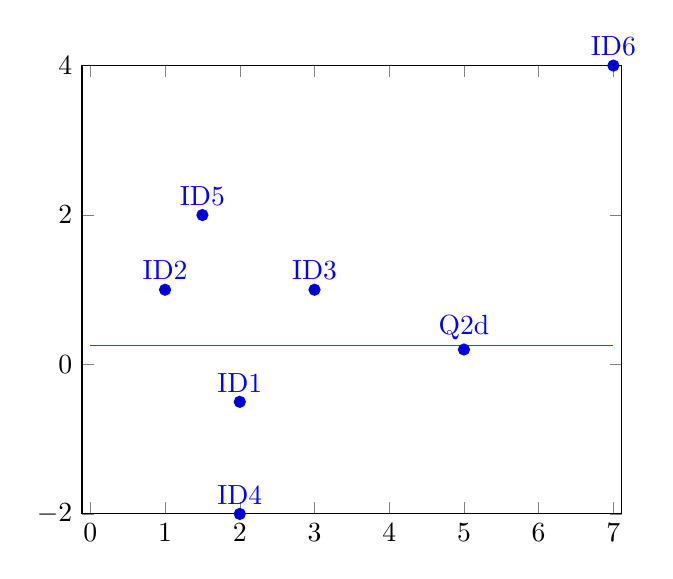
\begin{tikzpicture}
\begin{axis}[
    enlargelimits=false,
    axis equal
]
\addplot+[
    nodes near coords,
    only marks,
    point meta=explicit symbolic
]
table[meta=label] {
    x   y   label
    2  -0.5 ID1
    1   1   ID2
    3   1   ID3
    2  -2   ID4
    1.5 2   ID5
    7   4   ID6
    5   0.2 Q2d
};
\addplot [
    domain=0:7,
    samples=2,
    color=red,
]
{0.25};
\end{axis}
\end{tikzpicture}

\noindent The decision boundary is $y=0.25$.\\

\noindent \textbf{Question 2d}

\noindent Predict the test data point to be + class.

\section{Question 3}

\end{multicols*}
\end{document}